\documentclass[11pt]{amsart}

% Standard letter size paper with 1inch margins
\usepackage[letterpaper, margin=1in]{geometry}
\usepackage{booktabs} % For better looking tables
\usepackage{xcolor}
\usepackage{pifont}

% Useful packages 
\usepackage{amsmath, amssymb, amsthm, amsaddr}
\usepackage{enumerate, subcaption, graphicx, hyperref}
\usepackage{algorithm}
\usepackage{algpseudocode}
\usepackage{cite}
\usepackage{bm}

\newcommand{\I}{\mathrm{i}}
\DeclareMathOperator{\E}{e}

\title{AMATH 582: Homework 5}
\author{Hunter Lybbert} % first and last name

\address{Applied Mathematics Department, University of Washington, Seattle, WA 
\\ \texttt{hlybbert@uw.edu}}

\date{\today} % you can also just type the date instead of "\today"

\begin{document}

\maketitle

\begin{abstract}
    In this report we compare and analyze the merits of Convolutional Neural Networks (CNNs) against our previous work with the Fully Connected Network (FCN).
    An FCN with the best hyperparameter configuration from report 4 is trained with multiple different total number of weights.
    Additionally, hyper-parameter tuning is conducted for the CNN.
    Finally different CNNs are trained with different total numbers of weights but with the best hyperparameter configuration from the previous step.
    An analysis of the costs and benefits of these two models is presented, primarily focused on the number of weights, training time, and model accuracy on the test set.
\end{abstract}

\section{Introduction and Overview}\label{sec:Introduction}
In this report we continue our study of deep learning, the field of neural network based model architecture.

Again, our setup is a common supervised learning problem, given a collection of $N$ data points with labels in classification or target values in a regression setting $$\big\{(\bm{x_0}, y_0), (\bm{x_1}, y_1), ..., (\bm{x_{N-1}}, y_{N-1})\big\}.$$
The data is denoted as a matrix $X$ and a vector of target values or class labels $\bm y$.
We then are looking for a function $f$ which takes in the training data and most accurately predicts the target values or class labels, written in optimization form we are looking for the following
\begin{equation}
f_{MLE} = \underset{f}{\rm argmin } \frac 1 {2 \sigma^2}|| f(X) - \bm y ||_2^2
\label{eq:basic_ml_setup}
\end{equation}
where $\sigma^2$ is the variance of the normally distributed error terms $\epsilon \sim \mathcal N (0, \sigma^2)$ defined by $\epsilon_i = y_i - f(x_i)$
So said another way we are trying to minimize our errors in the classification task.
The specific class of functions $f$ to be considered to solve the problem is a neural network, specifically we evaluate and compare FCNs to CNNs.
We will treat the theoretical background of these methods in the next section \ref{sec:theory}.

Before proceeding, we would like to acknowledge the critical use of the following packages in our analysis.
Namely, Matplotlib was used to create all plots and animations \cite{Hunter:2007}.
Addiitonally, PyTorch \cite{Ansel_PyTorch_2_Faster_2024} was crucial for easily implementing the desired architecture while Ray Tune \cite{liaw2018tune} was used to help with hyper parameter tuning.

\section{Theoretical Background}\label{sec:theory}
For a general theoretical background on neural networks and basic hyperparameters please refer to the report from homework 4.
We presented our theoretical background clearly there.
Instead of repeating the information about gradient descent, back propogation, optimizers, learning rates, and dropout etc. in this report again, we will focus on the unique architectural considerations of a convolutional neural network.

\textbf{TODO: What is a convolution?}

\textbf{TODO: Present a visual representation of a convolutional layer}

\textbf{TODO: Present an example architecture, perhaps the one you used for your best CNN}

\subsection{Architecture}
\textbf{TODO: maybe reuse this section}

We will discuss what our own experiments revealed about weight initialization in our computational results section \ref{sec:results}.

\section{Algorithm Implementation and Development}\label{sec:algorithms}
In order to train a CNN we began by creating a model class using PyTorch's \cite{Ansel_PyTorch_2_Faster_2024} many built in methods and classes.
This time we manually experimented with different number of convolutional layers until we settled in on our basic architecture (3 convolutional layers and a fully connected layer).

I did not try to use Ray Tune \cite{liaw2018tune} again, but rather I generalized the model training python class I created in homework 4 to be able to apply it to both the CNN and FCN.
This generalizing of the python class led me to relearning a bit about python class inheritance and was a good exercise in trying to generalize my code.
This generalized class still managed the experiments for me and recorded results, total number of weights, training time, and other parameter settings to a \textit{json} file.
This allowed me to train many models over night and analyze the results the next day and refer back to them in the future as well.
It is all easy to use and very reproducible.

\textbf{TODO: Describe the architecture you ended up settling on (generally)}

Due to the large number of hyper parameters it is an overwhelming amount of information to specify in each plot for each loss or accuracy curve.
Therefore, I have labeled plots with experiment numbers and mean accuracy across test set.
For select models I will detail their exact configuration in the next section \ref{sec:results}, while others can be looked up in the repo directly on \href{https://github.com/hunter-lybbert/uw-central/blob/main/data_analysis/hw_05/experiments/experiments.json}{GitHub}.

\section{Computational Results}\label{sec:results}
We will primarily let the loss, accuracy curves, and hyperparameter configuration tables speak for themselves.
We have included a small sample of the results of our parameter tuning.
Please, see Figures \ref{fig:f0} and \ref{fig:f1} for visualizations of how batch normalization, weight initialization, optimizer choice, and learning rates effected the loss and accuracy curves throughout the training process.
After training our 300 plus models and inspecting which configurations produced a model with above $90\%$ test accuracy, we picked the configuration in \ref{tab:best_model}. We trained a model with this configuration for 5 repeated trials and report the test accuracy mean and standard deviation across trials.
We also repeated this process for the MNIST Digit classification problem from homework 3.
Our best model configuration aligns well with our theoretical background expectations for the optimizer, learning rate, dropout rates, batch normalization, and weight initialization.
A dropout rate around 0.5 was best.
Adam with a low learning rate barely edged out SGD with a larger of a learning rate.
We don't report on RMSprop here (due to space), however, it performed similar to Adam.

We also applied sklearn's $K$-nearest neighbors to this dataset and had a test accuracy of 0.8554 (with number of neighbors set to 5).
Varying the number of neighbors degraded the model slightly.

\begin{table}[h]
    \centering
    \begin{tabular}{|l|c|c|c|c|c|c|c|c|c|c|} % 'l' for left-aligned, 'c' for center-aligned columns
        \hline
        \textbf{Ep.}
        & \textbf{Arch} & \textbf{W. Init}
        & \textbf{B. Norm} & \textbf{Drop}
        & \textbf{Optim} & \textbf{lr}
	& \textbf{$\bm \mu$ (Test Acc)}
        & \textbf{$\bm \sigma$ (Test Acc)} \\ 
        \hline
        50 & [1024, 256]  & Kaiming & True & [0.5, 0.5] & Adam & 0.001 & 0.9030 \textcolor{red}{\ding{72}} & 0.0021 \\
        \hline
    \end{tabular}
    \caption{This was the configuration that was best from the last report in hw 04.
    Therefore it was the base setup for the FCN's trained in this hw 05, however, with the necessary adjustments due to weight count constraints.}
    \label{tab:best_model}
\end{table}

\begin{table}[h]
    \centering
    \begin{tabular}{|l|c|c|c|c|c|c|c|c|c|c|} % 'l' for left-aligned, 'c' for center-aligned columns
        \hline
        \textbf{ID} & \textbf{Model} & \textbf{Weights}
        & \textbf{Time} & \textbf{Ep.}
        & \textbf{Optim}
        & \textbf{lr} & \textbf{W. Init}  & \textbf{$\bm \mu$ (Test Acc)}
        & \textbf{$\bm \sigma$ (Test Acc)} \\
        \hline
        49 & CNN (100k) & 108,814 & 0:06:15 & 50 & Adam & 0.001 & Xavier & 0.9236 \textcolor{red}{\ding{72}} & 0.0167 \\
        \hline
        56 & CNN (10k) &   9,980 & 0:04:02 & 50 & Adam & 0.001 & Xavier & 0.9002 & 0.0229 \\
        \hline
        57 & CNN (20k) & 20,071 & 0:04:15 & 50 & Adam & 0.001 & Xavier & 0.9091 & 0.0151 \\
        \hline
        58 & CNN (50k) & 50,392 & 0:05:19 & 50 & Adam & 0.001 & Xavier & 0.9152 & 0.0188 \\
        \hline
        59 & FCN (50k) & 52,842 & 0:02:30 & 50 & Adam & 0.001 & Kaiming & 0.8802 & 0.0158 \\
        \hline
        60 & FCN (100k) & 109,770 & 0:02:32	 & 50 & Adam & 0.001 & Kaiming & 0.8889 & 0.0211 \\
        \hline
        61 & FCN (200k) & 202,974 & 0:02:32 & 50 & Adam & 0.001 & Kaiming & 0.8965 & 0.0188 \\
        \hline
    \end{tabular}
    \caption{
    After performing Hyperparameter tuning to determine the best settings for out CNNs, we trained models with 100k, 50k, 20k, and 10k weights.
    Using the configuration from Table \ref{tab:best_model} (best from homework 4) we trained 3 FCN's each with 200k, 100k, and 50k weights in each model.
    Notice that training time increases very rapidly for the CNN as the number of parameters increases, while the FCN training time is almost constant (at least at the scale and for the experiments we conducted.
    Finally, notice how even the smallest CNN outperforms the FCN on the test set accuracy, let alone how high the test accuracy is with the 100k weights CNN.}
    \label{tab:diff_weights}
\end{table}

\textbf{TODO: Talk about hyperparameter tuning for the CNN}
\textbf{TODO: Talk about the need for regularization and mitigating overfitting!}

\begin{figure}[h]
    \centering
    \begin{subfigure}{0.49\textwidth}
        \centering
        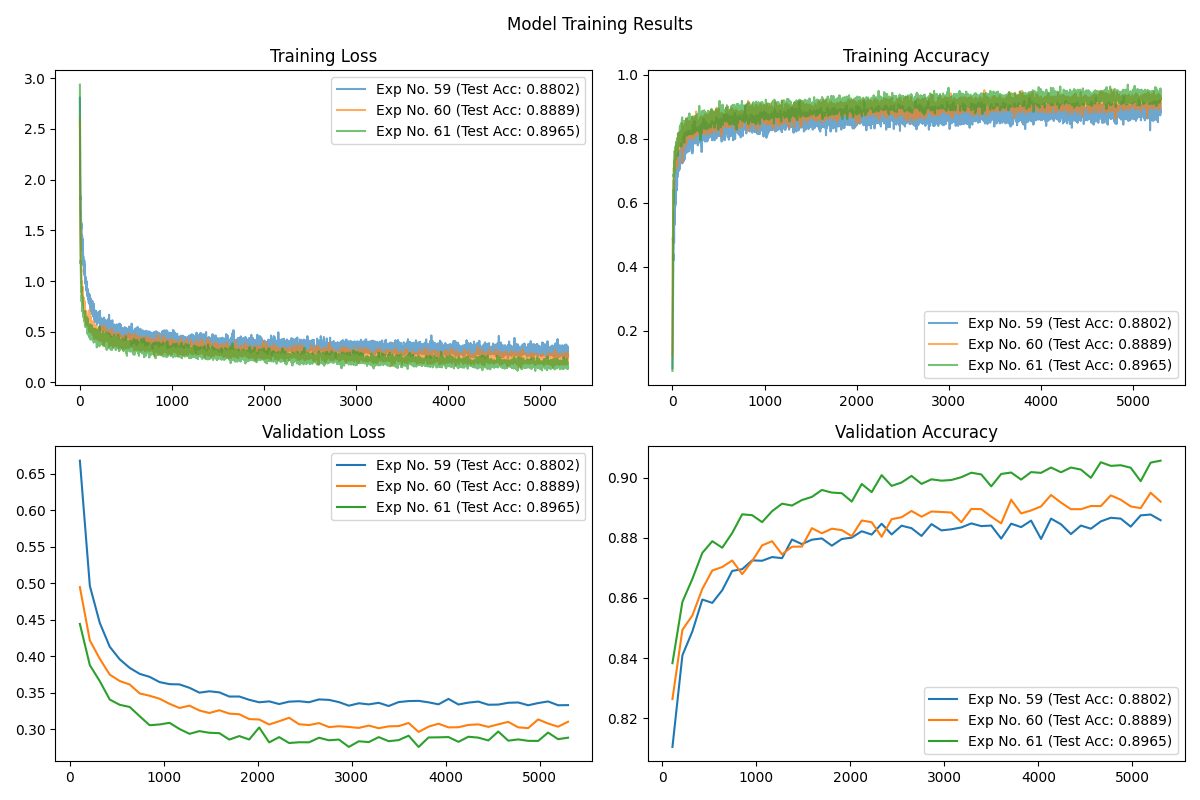
\includegraphics[width=.9\textwidth]{../visualizations/model_training_results_vis_2.png}
        \label{fig:image1}
    \end{subfigure}
    %\hspace{1mm}
    \begin{subfigure}{0.49\textwidth}
        \centering
        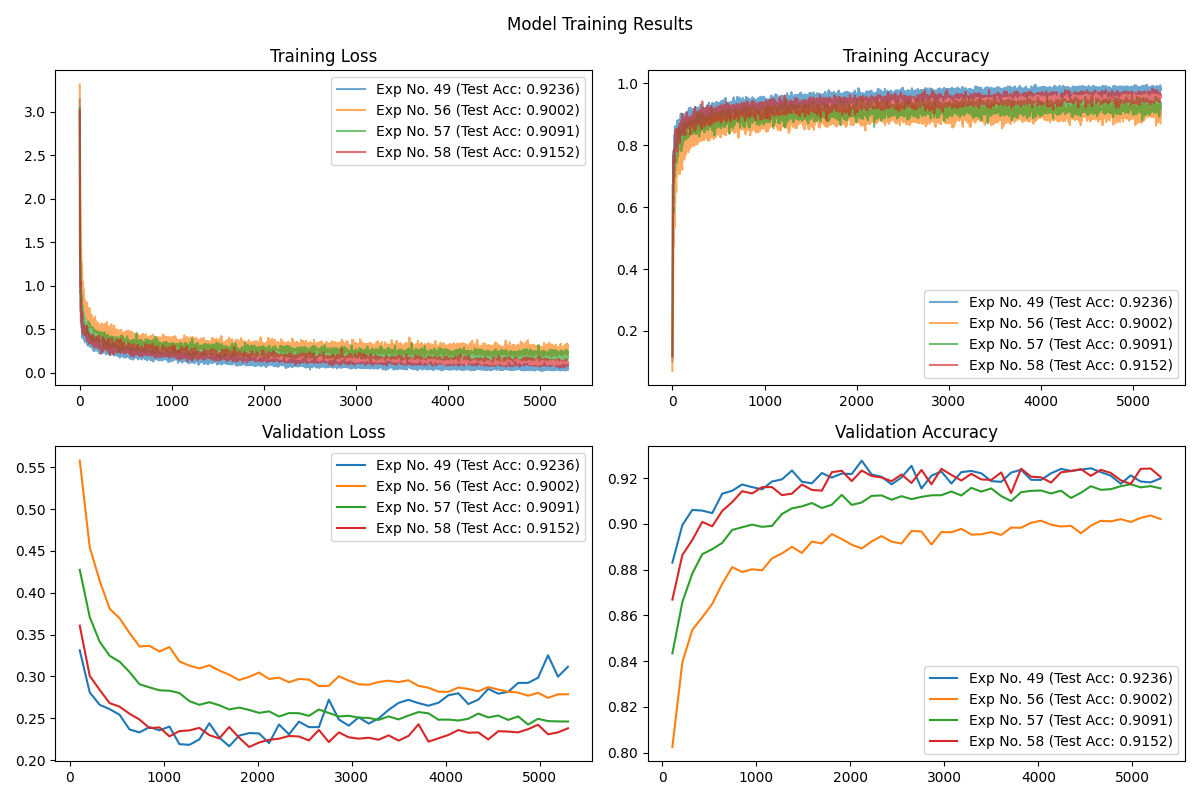
\includegraphics[width=.9\textwidth]{../visualizations/model_training_results_vis_3.png}
        \label{fig:image2}
    \end{subfigure}
    \caption{On the left we have the 3 different FCNs which are all the same except different total number of weights, compare to Table \ref{tab:diff_weights}.
    On the right are the 4 different CNNs trained with the same parameter settings except they vary the total number of weights, compare to Table \ref{tab:diff_weights}.}
    \label{fig:f0}
\end{figure}

\begin{table}[h]
    \centering
    \begin{tabular}{|l|c|c|c|c|c|c|c|c|c|c|} % 'l' for left-aligned, 'c' for center-aligned columns
        \hline
        \textbf{ID} & \textbf{Ep.}
        & \textbf{Arch} & \textbf{W. Init}
        & \textbf{B. Norm} & \textbf{Drop}
        & \textbf{Optim} & \textbf{lr}
	& \textbf{$\bm \mu$ (Test Acc)}
        & \textbf{$\bm \sigma$ (Test Acc)} \\ 
        \hline
        111 & 30 & [1024, 256]  & Xavier 	& True & [0.3, 0.5] & Adam & 0.001 & 0.8967 & 0.0222 \\
        \hline
        123 & 30 & [1024, 256]  & Random N. & True & [0.3, 0.2] & Adam & 0.001 & 0.8807 & 0.0202 \\
        \hline
        135 & 30 & [1024, 256]  & Kaiming 	& True & [0.1, 0.1] & Adam & 0.001 & 0.8912 & 0.0175 \\  
        \hline
    \end{tabular}
    \caption{\textbf{TODO: Convert this into something to talk about the hyper-parameter tuning of the CNNs}}
    \label{tab:tab0}
\end{table}

%\begin{table}[h]
%    \centering
%    \begin{tabular}{|l|c|c|c|c|c|c|c|c|c|c|} % 'l' for left-aligned, 'c' for center-aligned columns
%        \hline
%        \textbf{ID} & \textbf{Ep.}
%        & \textbf{Arch} & \textbf{W. Init}
%        & \textbf{B. Norm} & \textbf{Drop}
%        & \textbf{Optim} & \textbf{lr}
%	& \textbf{$\bm \mu$ (Test Acc)}
%        & \textbf{$\bm \sigma$ (Test Acc)} \\ 
%        \hline
%        117 & 30 & [1024, 256]  & Xavier 		& False & [0.1, 0.1] & Adam & 0.001 & 0.8976 & 0.0175 \\
%        \hline
%        129 & 30 & [1024, 256]  & Random N. 	& False & [0.5, 0.3] & Adam & 0.001 & 0.7372 & 0.0335 \\
%        \hline
%        141 & 30 & [1024, 256]  & Kaiming 		& False & [0.2, 0.5] & Adam & 0.001 & 0.8978 & 0.0251 \\  
%        \hline
%    \end{tabular}
%    \caption{This is a set of 3 experiments where all things are constant except the weight initializations differ.
%    Additionally it can be compared to \ref{tab:tab0} since these are the same as those experiments just without Batch Normalization.
%    See the right hand side of Figure \ref{fig:f0} for a visual of the training and validation loss and accuracy curves.}
%    \label{tab:tab1}
%\end{table}

\begin{figure}[h]
	\centering
	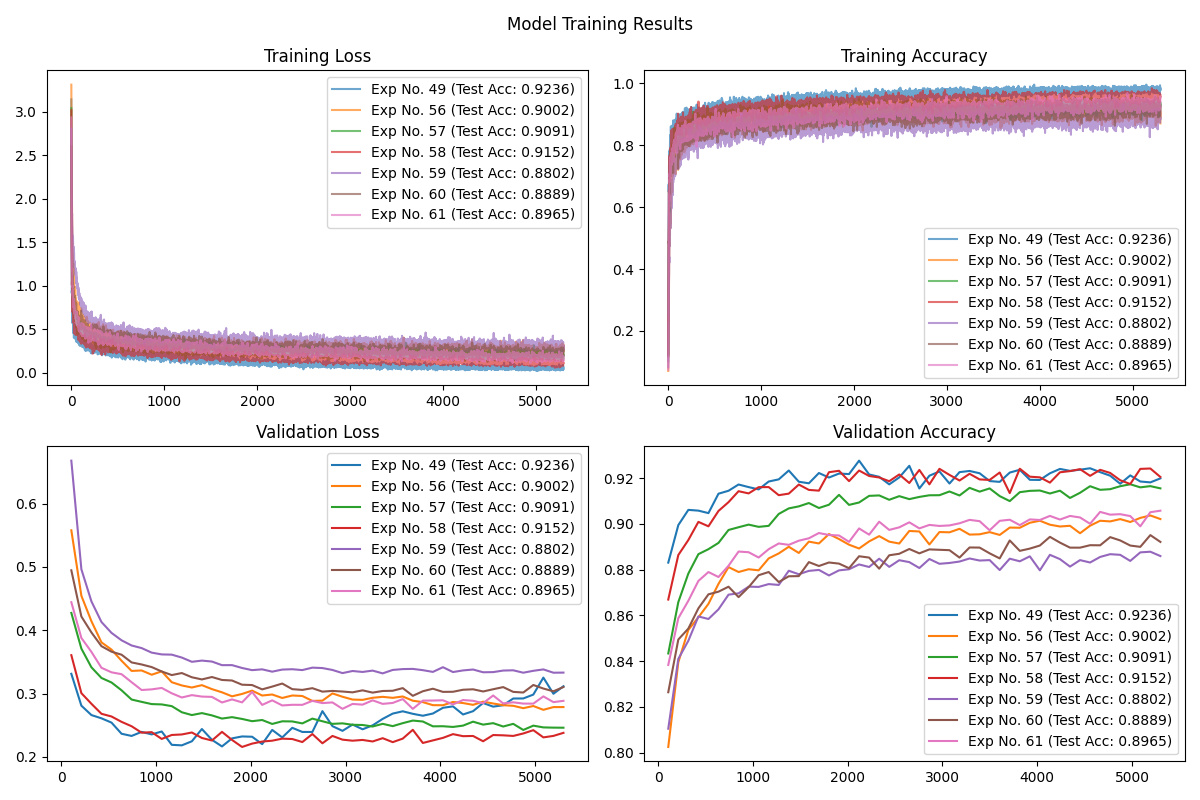
\includegraphics[width=.6\textwidth]{../visualizations/model_training_results_vis_1.png}
\caption{This is a visualization of all of all models in Table \ref{tab:diff_weights}.
	They were visualized separately in Figure \ref{fig:f0}.}
    \label{fig:f1}
\end{figure}

%\begin{table}[h]
%    \centering
%    \begin{tabular}{|l|c|c|c|c|c|c|c|c|c|c|} % 'l' for left-aligned, 'c' for center-aligned columns
%        \hline
%        \textbf{ID} & \textbf{Ep.}
%        & \textbf{Arch} & \textbf{W. Init}
%        & \textbf{B. Norm} & \textbf{Drop}
%        & \textbf{Optim} & \textbf{lr}
%	& \textbf{$\bm \mu$ (Test Acc)}
%        & \textbf{$\bm \sigma$ (Test Acc)} \\ 
%        \hline
%        109 & 30 & [1024, 256]  & Xavier & True & [0.1, 0.1] & Adam & 0.01 & 0.8906 & 0.0214 \\
%        \hline
%        111 & 30 & [1024, 256]  & Xavier & True & [0.3, 0.5] & Adam & 0.001 & 0.8967 & 0.0222 \\
%        \hline
%        113 & 30 & [1024, 256]  & Xavier & True & [0.5, 0.2] & Adam & 0.0001 & 0.8933 & 0.0189 \\  
%        \hline
%    \end{tabular}
%    \caption{Here all things are constant, including the Adam optimizer, we only vary the learning rate.
%    See the left hand side of Figure \ref{fig:f1} for the visualization of this.
%    Compare this to Table \ref{tab:tab3} as well to see the same learning rates and config but with SGD.}
%    \label{tab:tab2}
%\end{table}

%\begin{table}[h]
%    \centering
%    \begin{tabular}{|l|c|c|c|c|c|c|c|c|c|c|} % 'l' for left-aligned, 'c' for center-aligned columns
%        \hline
%        \textbf{ID} & \textbf{Ep.}
%        & \textbf{Arch} & \textbf{W. Init}
%        & \textbf{B. Norm} & \textbf{Drop}
%        & \textbf{Optim} & \textbf{lr}
%	& \textbf{$\bm \mu$ (Test Acc)}
%        & \textbf{$\bm \sigma$ (Test Acc)} \\ 
%        \hline
%        108 & 30 & [1024, 256]  & Xavier & True & [0.3, 0.1] & SGD & 0.01 & 0.8958 & 0.0196 \\
%        \hline
%        110 & 30 & [1024, 256]  & Xavier & True & [0.2, 0.1] & SGD & 0.001 & 0.8956 & 0.0239 \\
%        \hline
%        112 & 30 & [1024, 256]  & Xavier & True & [0.5, 0.1] & SGD & 0.0001 & 0.8191 & 0.0293 \\  
%        \hline
%    \end{tabular}
%    \caption{
%    Again all things are constant, including the SGD optimizer, we only vary the learning rate.
%    See the right hand side of Figure \ref{fig:f1} for the visualization of this.
%    Compare this to Table \ref{tab:tab2} as well to see the same learning rates and config but with Adam.
%    }
%    \label{tab:tab3}
%\end{table}


\section{Summary and Conclusions}\label{sec:conclusions} 
\textbf{TODO: Conclude which model you would use when based on needing it to train quickly, visual data, etc. }
The method we settled on limited how we could convey the results here in the report, though it recorded thorough information for later reference on \href{https://github.com/hunter-lybbert/uw-central/blob/main/data_analysis/hw_04/experiments/experiments.json}{GitHub}
This was an excellent introductory experience into building, training, and evaluating a neural network.

\section*{Acknowledgements}
The author is thankful to Jaxon Tuggle for offering regular feedback and counsel when interpreting results and clarifying the implications and merits throughout the hyperparameter tuning process.
We would also like to thank Professor Eli Shlizerman for carefully instructing us in class.

\bibliographystyle{abbrv}
\bibliography{references_hw5} % make sure this matches the .bib file for your corresponding document. You also have to maintain your references in the .bib file 

\end{document}
